\subsection{Complete per-task and per-configuration scores}
\label{sec:full-scores}

Tables~\ref{tab:full-scores-easy}--\ref{tab:full-scores-impossible} report all 200 runs and all four reported quantities, comprising 200 composite scores and 600 component values. Standard is the primary comparison using the same model backbone; Record and Brief are workflow ablations. Every task has one result for each configuration.

Composite scores are displayed to four decimal places and component scores to six decimal places. The accompanying \texttt{cloudrabench\_200\_run\_scores.csv} retains the original full-precision numeric strings. Accordingly, recomputing the weighted composite from the displayed component values can differ from the separately rounded composite in the last shown digit. The printed scientific self-consistency score is the graded component, distinct from the separate all-or-none scientific acceptance decision.

\begingroup
\small
\setlength{\tabcolsep}{6pt}
\renewcommand{\arraystretch}{1.05}
\begin{longtable}{@{}llrrrr@{}}
\caption{Complete Easy-tier results for all four configurations. $S$: composite score; $G$: graph structure; $SC$: scientific self-consistency score; $A$: accuracy.}\label{tab:full-scores-easy}\\
\toprule
Task & Configuration & $S$ & $G$ & $SC$ & $A$ \\
\midrule
\endfirsthead
\multicolumn{6}{l}{\tablename\ \thetable\ (continued)}\\
\toprule
Task & Configuration & $S$ & $G$ & $SC$ & $A$ \\
\midrule
\endhead
\midrule
\multicolumn{6}{r}{Continued on the next page}\\
\endfoot
\bottomrule
\endlastfoot
D1 & Guided & 0.8200 & 1.000000 & 1.000000 & 0.700000 \\
D1 & Standard & 0.8291 & 0.791667 & 0.500000 & 0.999960 \\
D1 & Record & 0.7992 & 0.791667 & 1.000000 & 0.700000 \\
D1 & Brief & 0.7450 & 1.000000 & 0.750000 & 0.700000 \\
\addlinespace[3pt]
D3 & Guided & 0.7450 & 1.000000 & 0.750000 & 0.700000 \\
D3 & Standard & 0.9247 & 1.000000 & 0.750000 & 0.999496 \\
D3 & Record & 0.7940 & 0.944444 & 0.350000 & 0.990939 \\
D3 & Brief & 0.7283 & 0.833333 & 0.750000 & 0.700000 \\
\addlinespace[3pt]
D4 & Guided & 0.9250 & 1.000000 & 0.750000 & 0.999982 \\
D4 & Standard & 0.8500 & 1.000000 & 0.500000 & 0.999982 \\
D4 & Record & 0.9104 & 1.000000 & 0.750000 & 0.975699 \\
D4 & Brief & 0.9049 & 0.944444 & 0.750000 & 0.975698 \\
\addlinespace[3pt]
E1 & Guided & 1.0000 & 1.000000 & 1.000000 & 0.999972 \\
E1 & Standard & 0.7828 & 0.777778 & 0.350000 & 0.999973 \\
E1 & Record & 1.0000 & 1.000000 & 1.000000 & 0.999973 \\
E1 & Brief & 1.0000 & 1.000000 & 1.000000 & 0.999973 \\
\addlinespace[3pt]
F1 & Guided & 0.9417 & 0.916667 & 0.833333 & 1.000000 \\
F1 & Standard & 0.0333 & 0.333333 & 0.000000 & 0.000000 \\
F1 & Record & 0.9917 & 0.916667 & 1.000000 & 1.000000 \\
F1 & Brief & 0.9117 & 0.916667 & 0.750000 & 0.991654 \\
\addlinespace[3pt]
F4 & Guided & 0.3601 & 0.600902 & 1.000000 & 0.000000 \\
F4 & Standard & 0.9083 & 0.833333 & 0.750000 & 0.999999 \\
F4 & Record & 0.9167 & 0.916667 & 0.750000 & 0.999999 \\
F4 & Brief & 0.3601 & 0.600902 & 1.000000 & 0.000000 \\
\addlinespace[3pt]
G2 & Guided & 0.2389 & 0.888889 & 0.500000 & 0.000000 \\
G2 & Standard & 0.7769 & 1.000000 & 0.500000 & 0.878159 \\
G2 & Record & 0.7769 & 1.000000 & 0.500000 & 0.878161 \\
G2 & Brief & 0.8500 & 1.000000 & 0.500000 & 0.999986 \\
\addlinespace[3pt]
G3 & Guided & 0.9832 & 0.833333 & 1.000000 & 0.999830 \\
G3 & Standard & 0.1417 & 0.666667 & 0.250000 & 0.000000 \\
G3 & Record & 0.9832 & 0.833333 & 1.000000 & 0.999830 \\
G3 & Brief & 0.9749 & 0.750000 & 1.000000 & 0.999833 \\
\addlinespace[3pt]
L1 & Guided & 0.9999 & 1.000000 & 1.000000 & 0.999899 \\
L1 & Standard & 0.9749 & 1.000000 & 0.916667 & 0.999900 \\
L1 & Record & 0.9999 & 1.000000 & 1.000000 & 0.999900 \\
L1 & Brief & 0.9999 & 1.000000 & 1.000000 & 0.999899 \\
\addlinespace[3pt]
L2 & Guided & 0.7450 & 1.000000 & 0.750000 & 0.700000 \\
L2 & Standard & 0.6700 & 1.000000 & 0.500000 & 0.700000 \\
L2 & Record & 0.8549 & 1.000000 & 0.750000 & 0.883231 \\
L2 & Brief & 0.8799 & 1.000000 & 0.833333 & 0.883239 \\
\addlinespace[3pt]
M1 & Guided & 0.9478 & 1.000000 & 1.000000 & 0.913062 \\
M1 & Standard & 0.7526 & 1.000000 & 0.350000 & 0.912639 \\
M1 & Record & 0.9476 & 1.000000 & 1.000000 & 0.912639 \\
M1 & Brief & 0.9476 & 1.000000 & 1.000000 & 0.912638 \\
\addlinespace[3pt]
M14 & Guided & 1.0000 & 1.000000 & 1.000000 & 1.000000 \\
M14 & Standard & 0.8050 & 1.000000 & 0.350000 & 1.000000 \\
M14 & Record & 1.0000 & 1.000000 & 1.000000 & 1.000000 \\
M14 & Brief & 1.0000 & 1.000000 & 1.000000 & 1.000000 \\
\addlinespace[3pt]
M15 & Guided & 1.0000 & 1.000000 & 1.000000 & 0.999999 \\
M15 & Standard & 1.0000 & 1.000000 & 1.000000 & 0.999999 \\
M15 & Record & 1.0000 & 1.000000 & 1.000000 & 0.999983 \\
M15 & Brief & 1.0000 & 1.000000 & 1.000000 & 0.999999 \\
\addlinespace[3pt]
M16 & Guided & 0.9748 & 1.000000 & 0.916667 & 0.999691 \\
M16 & Standard & 0.9998 & 1.000000 & 1.000000 & 0.999692 \\
M16 & Record & 0.9915 & 0.916667 & 1.000000 & 0.999694 \\
M16 & Brief & 0.9998 & 1.000000 & 1.000000 & 0.999692 \\
\addlinespace[3pt]
M17 & Guided & 0.9999 & 1.000000 & 1.000000 & 0.999914 \\
M17 & Standard & 0.0778 & 0.777778 & 0.000000 & 0.000000 \\
M17 & Record & 0.9999 & 1.000000 & 1.000000 & 0.999914 \\
M17 & Brief & 0.9999 & 1.000000 & 1.000000 & 0.999914 \\
\addlinespace[3pt]
M3 & Guided & 1.0000 & 1.000000 & 1.000000 & 0.999996 \\
M3 & Standard & 1.0000 & 1.000000 & 1.000000 & 0.999996 \\
M3 & Record & 1.0000 & 1.000000 & 1.000000 & 0.999996 \\
M3 & Brief & 1.0000 & 1.000000 & 1.000000 & 0.999996 \\
\addlinespace[3pt]
M8 & Guided & 0.9996 & 1.000000 & 1.000000 & 0.999335 \\
M8 & Standard & 0.9996 & 1.000000 & 1.000000 & 0.999339 \\
M8 & Record & 0.9996 & 1.000000 & 1.000000 & 0.999294 \\
M8 & Brief & 0.9996 & 1.000000 & 1.000000 & 0.999294 \\
\addlinespace[3pt]
P2 & Guided & 1.0000 & 1.000000 & 1.000000 & 0.999948 \\
P2 & Standard & 0.9833 & 0.833333 & 1.000000 & 0.999947 \\
P2 & Record & 0.9833 & 0.833333 & 1.000000 & 0.999947 \\
P2 & Brief & 0.9750 & 1.000000 & 0.916667 & 0.999947 \\
\addlinespace[3pt]
P3 & Guided & 0.9380 & 1.000000 & 1.000000 & 0.896739 \\
P3 & Standard & 0.1000 & 1.000000 & 0.000000 & 0.000000 \\
P3 & Record & 0.9380 & 1.000000 & 1.000000 & 0.896735 \\
P3 & Brief & 0.8309 & 1.000000 & 1.000000 & 0.718109 \\
\addlinespace[3pt]
X1 & Guided & 0.9999 & 1.000000 & 1.000000 & 0.999916 \\
X1 & Standard & 0.9999 & 1.000000 & 1.000000 & 0.999914 \\
X1 & Record & 0.9999 & 1.000000 & 1.000000 & 0.999916 \\
X1 & Brief & 0.9999 & 1.000000 & 1.000000 & 0.999914 \\
\addlinespace[3pt]
\end{longtable}
\endgroup

\begingroup
\small
\setlength{\tabcolsep}{6pt}
\renewcommand{\arraystretch}{1.05}
\begin{longtable}{@{}llrrrr@{}}
\caption{Complete Normal-tier results for all four configurations. $S$: composite score; $G$: graph structure; $SC$: scientific self-consistency score; $A$: accuracy.}\label{tab:full-scores-normal}\\
\toprule
Task & Configuration & $S$ & $G$ & $SC$ & $A$ \\
\midrule
\endfirsthead
\multicolumn{6}{l}{\tablename\ \thetable\ (continued)}\\
\toprule
Task & Configuration & $S$ & $G$ & $SC$ & $A$ \\
\midrule
\endhead
\midrule
\multicolumn{6}{r}{Continued on the next page}\\
\endfoot
\bottomrule
\endlastfoot
NB1 & Guided & 0.9628 & 0.628571 & 1.000000 & 0.999972 \\
NB1 & Standard & 0.9128 & 0.628571 & 0.833333 & 0.999970 \\
NB1 & Record & 0.8625 & 0.600000 & 0.675000 & 0.999972 \\
NB1 & Brief & 0.9900 & 0.900000 & 1.000000 & 0.999972 \\
\addlinespace[3pt]
NI1 & Guided & 0.9958 & 1.000000 & 1.000000 & 0.993046 \\
NI1 & Standard & 0.6196 & 0.946119 & 0.350000 & 0.700000 \\
NI1 & Record & 0.7767 & 0.816667 & 0.916667 & 0.700000 \\
NI1 & Brief & 0.9889 & 1.000000 & 1.000000 & 0.981480 \\
\addlinespace[3pt]
NI5 & Guided & 0.7715 & 0.928571 & 1.000000 & 0.631094 \\
NI5 & Standard & 0.3136 & 0.571429 & 0.675000 & 0.089878 \\
NI5 & Record & 0.1542 & 0.442375 & 0.366667 & 0.000000 \\
NI5 & Brief & 0.3571 & 0.571429 & 1.000000 & 0.000000 \\
\addlinespace[3pt]
NQ1 & Guided & 0.7395 & 0.945455 & 0.750000 & 0.700000 \\
NQ1 & Standard & 0.9040 & 0.797980 & 0.750000 & 0.998691 \\
NQ1 & Record & 0.7131 & 0.680808 & 0.750000 & 0.700000 \\
NQ1 & Brief & 0.1731 & 0.680808 & 0.350000 & 0.000000 \\
\addlinespace[3pt]
NQ5 & Guided & 0.7075 & 1.000000 & 0.625000 & 0.700000 \\
NQ5 & Standard & 0.7510 & 0.920000 & 0.550000 & 0.823369 \\
NQ5 & Record & 0.8725 & 1.000000 & 0.625000 & 0.974999 \\
NQ5 & Brief & 0.7810 & 1.000000 & 0.625000 & 0.822502 \\
\addlinespace[3pt]
NR1 & Guided & 0.6167 & 0.666667 & 0.833333 & 0.500000 \\
NR1 & Standard & 0.1643 & 0.592593 & 0.350000 & 0.000002 \\
NR1 & Record & 0.5378 & 0.777778 & 0.533333 & 0.500000 \\
NR1 & Brief & 0.6142 & 0.666667 & 0.875000 & 0.475000 \\
\addlinespace[3pt]
NU3 & Guided & 0.5527 & 0.776832 & 0.916667 & 0.333330 \\
NU3 & Standard & 0.3621 & 0.571429 & 0.350000 & 0.333330 \\
NU3 & Record & 0.4071 & 0.571429 & 0.500000 & 0.333330 \\
NU3 & Brief & 0.6829 & 0.828571 & 0.666667 & 0.666657 \\
\addlinespace[3pt]
NU5 & Guided & 0.3518 & 0.642857 & 0.958333 & 0.000000 \\
NU5 & Standard & 0.2654 & 0.904762 & 0.116667 & 0.233136 \\
NU5 & Record & 0.2966 & 0.779762 & 0.233333 & 0.247741 \\
NU5 & Brief & 0.1983 & 0.662546 & 0.440000 & 0.000000 \\
\addlinespace[3pt]
NU6 & Guided & 0.6719 & 1.000000 & 0.937500 & 0.484393 \\
NU6 & Standard & 0.6892 & 0.816667 & 0.625000 & 0.700000 \\
NU6 & Record & 0.1450 & 0.400000 & 0.350000 & 0.000000 \\
NU6 & Brief & 0.3400 & 0.400000 & 1.000000 & 0.000000 \\
\addlinespace[3pt]
NY3 & Guided & 1.0000 & 1.000000 & 1.000000 & 0.999998 \\
NY3 & Standard & 0.7485 & 0.857143 & 0.616667 & 0.796239 \\
NY3 & Record & 0.5217 & 0.716855 & 0.833333 & 0.333333 \\
NY3 & Brief & 0.7312 & 0.761905 & 0.783333 & 0.700000 \\
\addlinespace[3pt]
\end{longtable}
\endgroup

\begingroup
\small
\setlength{\tabcolsep}{6pt}
\renewcommand{\arraystretch}{1.05}
\begin{longtable}{@{}llrrrr@{}}
\caption{Complete Hard-tier results for all four configurations. $S$: composite score; $G$: graph structure; $SC$: scientific self-consistency score; $A$: accuracy.}\label{tab:full-scores-hard}\\
\toprule
Task & Configuration & $S$ & $G$ & $SC$ & $A$ \\
\midrule
\endfirsthead
\multicolumn{6}{l}{\tablename\ \thetable\ (continued)}\\
\toprule
Task & Configuration & $S$ & $G$ & $SC$ & $A$ \\
\midrule
\endhead
\midrule
\multicolumn{6}{r}{Continued on the next page}\\
\endfoot
\bottomrule
\endlastfoot
HA1 & Guided & 0.9625 & 1.000000 & 0.875000 & 1.000000 \\
HA1 & Standard & 0.1000 & 1.000000 & 0.000000 & 0.000000 \\
HA1 & Record & 0.9250 & 1.000000 & 0.750000 & 1.000000 \\
HA1 & Brief & 0.9250 & 1.000000 & 0.750000 & 1.000000 \\
\addlinespace[3pt]
HA6 & Guided & 0.9750 & 1.000000 & 0.916667 & 1.000000 \\
HA6 & Standard & 0.9625 & 1.000000 & 0.875000 & 1.000000 \\
HA6 & Record & 0.9750 & 1.000000 & 0.916667 & 1.000000 \\
HA6 & Brief & 0.9750 & 1.000000 & 0.916667 & 1.000000 \\
\addlinespace[3pt]
HA8 & Guided & 0.9625 & 1.000000 & 0.875000 & 0.999961 \\
HA8 & Standard & 0.6250 & 1.000000 & 0.350000 & 0.700000 \\
HA8 & Record & 0.9250 & 1.000000 & 0.750000 & 0.999961 \\
HA8 & Brief & 0.7450 & 1.000000 & 0.750000 & 0.700000 \\
\addlinespace[3pt]
HB1 & Guided & 0.9325 & 0.700000 & 0.875000 & 1.000000 \\
HB1 & Standard & 0.8250 & 0.750000 & 0.500000 & 1.000000 \\
HB1 & Record & 0.9700 & 0.700000 & 1.000000 & 1.000000 \\
HB1 & Brief & 0.9800 & 0.800000 & 1.000000 & 1.000000 \\
\addlinespace[3pt]
HB10 & Guided & 0.9995 & 1.000000 & 1.000000 & 0.999225 \\
HB10 & Standard & 0.9928 & 0.932344 & 1.000000 & 0.999217 \\
HB10 & Record & 0.8044 & 0.999011 & 0.350000 & 0.999226 \\
HB10 & Brief & 0.7845 & 0.800000 & 0.350000 & 0.999239 \\
\addlinespace[3pt]
HD2 & Guided & 0.7867 & 0.666667 & 1.000000 & 0.700000 \\
HD2 & Standard & 0.6977 & 0.666667 & 0.350000 & 0.876795 \\
HD2 & Record & 0.5950 & 1.000000 & 0.250000 & 0.700000 \\
HD2 & Brief & 0.6699 & 0.999176 & 0.500000 & 0.700000 \\
\addlinespace[3pt]
HF1 & Guided & 0.9742 & 0.741868 & 1.000000 & 1.000000 \\
HF1 & Standard & 0.3425 & 0.799505 & 0.875000 & 0.000000 \\
HF1 & Record & 0.9072 & 0.821728 & 0.750000 & 1.000000 \\
HF1 & Brief & 0.2937 & 0.687405 & 0.750000 & 0.000000 \\
\addlinespace[3pt]
HH1 & Guided & 0.9838 & 1.000000 & 1.000000 & 0.973067 \\
HH1 & Standard & 0.8338 & 1.000000 & 0.500000 & 0.973064 \\
HH1 & Record & 0.7888 & 1.000000 & 0.350000 & 0.973066 \\
HH1 & Brief & 0.9838 & 1.000000 & 1.000000 & 0.973066 \\
\addlinespace[3pt]
HI1 & Guided & 0.9999 & 0.999176 & 1.000000 & 0.999998 \\
HI1 & Standard & 0.7032 & 0.332509 & 0.233333 & 0.999998 \\
HI1 & Record & 0.9350 & 0.999588 & 0.783333 & 0.999998 \\
HI1 & Brief & 0.9999 & 0.999176 & 1.000000 & 0.999998 \\
\addlinespace[3pt]
HL1 & Guided & 0.9999 & 0.999176 & 1.000000 & 0.999999 \\
HL1 & Standard & 0.8050 & 1.000000 & 0.350000 & 0.999999 \\
HL1 & Record & 0.8972 & 0.722222 & 0.750000 & 0.999995 \\
HL1 & Brief & 0.9250 & 1.000000 & 0.750000 & 0.999999 \\
\addlinespace[3pt]
\end{longtable}
\endgroup

\begingroup
\small
\setlength{\tabcolsep}{6pt}
\renewcommand{\arraystretch}{1.05}
\begin{longtable}{@{}llrrrr@{}}
\caption{Complete Impossible-tier results for all four configurations. $S$: composite score; $G$: graph structure; $SC$: scientific self-consistency score; $A$: accuracy.}\label{tab:full-scores-impossible}\\
\toprule
Task & Configuration & $S$ & $G$ & $SC$ & $A$ \\
\midrule
\endfirsthead
\multicolumn{6}{l}{\tablename\ \thetable\ (continued)}\\
\toprule
Task & Configuration & $S$ & $G$ & $SC$ & $A$ \\
\midrule
\endhead
\midrule
\multicolumn{6}{r}{Continued on the next page}\\
\endfoot
\bottomrule
\endlastfoot
IA1 & Guided & 0.1717 & 0.666667 & 0.350000 & 0.000000 \\
IA1 & Standard & 0.1717 & 0.666667 & 0.350000 & 0.000000 \\
IA1 & Record & 0.1717 & 0.666667 & 0.350000 & 0.000000 \\
IA1 & Brief & 1.0000 & 1.000000 & 1.000000 & 1.000000 \\
\addlinespace[3pt]
IA5 & Guided & 0.4000 & 1.000000 & 1.000000 & 0.000000 \\
IA5 & Standard & 0.1417 & 0.666667 & 0.250000 & 0.000000 \\
IA5 & Record & 0.4000 & 1.000000 & 1.000000 & 0.000000 \\
IA5 & Brief & 0.3667 & 0.666667 & 1.000000 & 0.000000 \\
\addlinespace[3pt]
IA7 & Guided & 0.2583 & 0.333333 & 0.750000 & 0.000000 \\
IA7 & Standard & 0.1383 & 0.333333 & 0.350000 & 0.000000 \\
IA7 & Record & 0.2583 & 0.333333 & 0.750000 & 0.000000 \\
IA7 & Brief & 0.2583 & 0.333333 & 0.750000 & 0.000000 \\
\addlinespace[3pt]
IA9 & Guided & 0.3667 & 0.666667 & 1.000000 & 0.000000 \\
IA9 & Standard & 0.2583 & 0.333333 & 0.750000 & 0.000000 \\
IA9 & Record & 0.3667 & 0.666667 & 1.000000 & 0.000000 \\
IA9 & Brief & 0.9333 & 0.333333 & 1.000000 & 1.000000 \\
\addlinespace[3pt]
IB9 & Guided & 0.8200 & 1.000000 & 1.000000 & 0.700000 \\
IB9 & Standard & 0.1800 & 0.750000 & 0.350000 & 0.000000 \\
IB9 & Record & 0.5450 & 0.200000 & 0.750000 & 0.500000 \\
IB9 & Brief & 0.7700 & 1.000000 & 0.833333 & 0.700000 \\
\addlinespace[3pt]
IC3 & Guided & 0.4000 & 1.000000 & 1.000000 & 0.000000 \\
IC3 & Standard & 0.1833 & 0.333333 & 0.500000 & 0.000000 \\
IC3 & Record & 0.2167 & 0.666667 & 0.500000 & 0.000000 \\
IC3 & Brief & 0.4000 & 1.000000 & 1.000000 & 0.000000 \\
\addlinespace[3pt]
ID2 & Guided & 0.3339 & 0.339244 & 1.000000 & 0.000000 \\
ID2 & Standard & 0.0000 & 0.000000 & 0.000000 & 0.000000 \\
ID2 & Record & 0.0000 & 0.000000 & 0.000000 & 0.000000 \\
ID2 & Brief & 0.1839 & 0.339244 & 0.500000 & 0.000000 \\
\addlinespace[3pt]
IE2 & Guided & 0.3333 & 0.333333 & 1.000000 & 0.000000 \\
IE2 & Standard & 0.0333 & 0.333333 & 0.000000 & 0.000000 \\
IE2 & Record & 0.0333 & 0.333333 & 0.000000 & 0.000000 \\
IE2 & Brief & 0.1833 & 0.333333 & 0.500000 & 0.000000 \\
\addlinespace[3pt]
IF3 & Guided & 0.3667 & 0.666667 & 1.000000 & 0.000000 \\
IF3 & Standard & 0.3667 & 0.666667 & 1.000000 & 0.000000 \\
IF3 & Record & 0.3333 & 0.333333 & 1.000000 & 0.000000 \\
IF3 & Brief & 0.4000 & 1.000000 & 1.000000 & 0.000000 \\
\addlinespace[3pt]
IG8 & Guided & 1.0000 & 1.000000 & 1.000000 & 1.000000 \\
IG8 & Standard & 1.0000 & 1.000000 & 1.000000 & 1.000000 \\
IG8 & Record & 0.0000 & 0.000000 & 0.000000 & 0.000000 \\
IG8 & Brief & 0.3339 & 0.339329 & 1.000000 & 0.000000 \\
\addlinespace[3pt]
\end{longtable}
\endgroup


\subsection{Expanded task-score matrices}
The two vector panels below expand the complete per-task score view for reading alongside the exact values in Tables~\ref{tab:full-scores-easy}--\ref{tab:full-scores-impossible}. Both use the same color scale and configuration order as the manuscript.
\begin{figure}[!t]
\centering
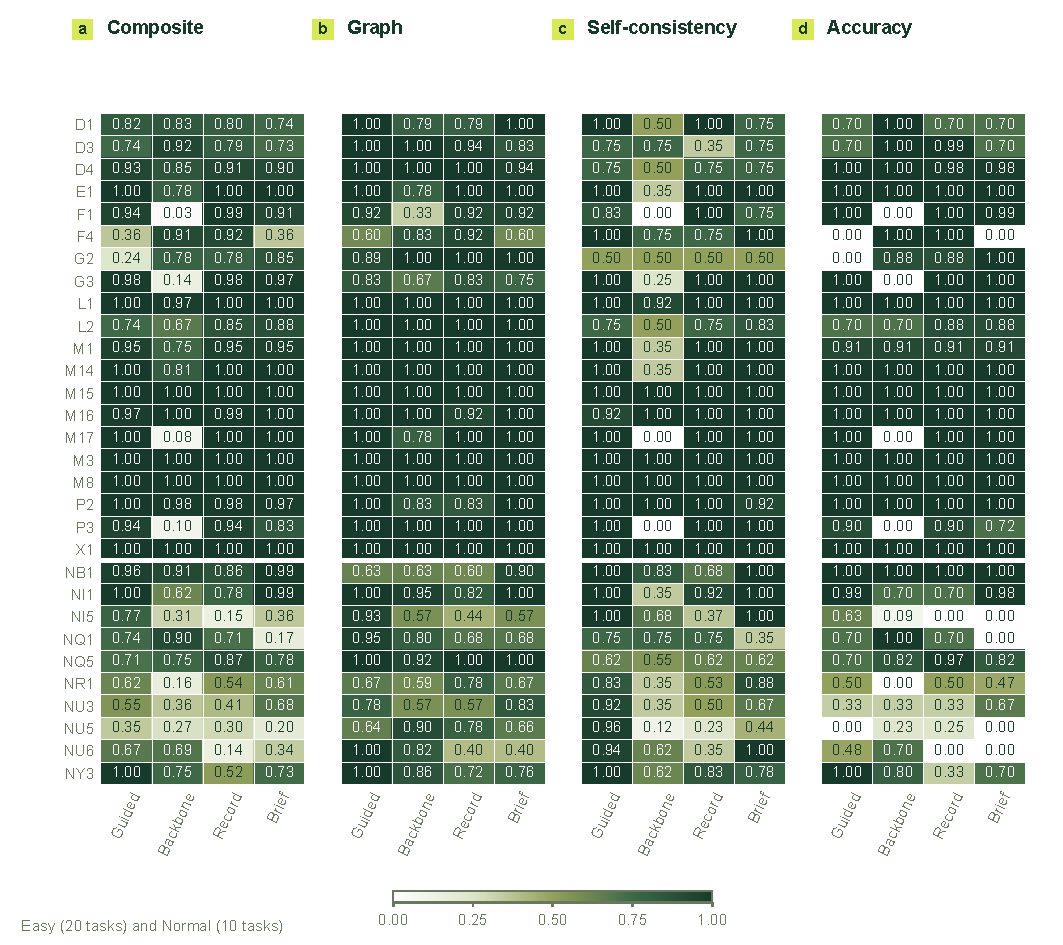
\includegraphics[width=\textwidth]{figures/bench_tasks.pdf}
\caption{All Easy and Normal task scores. Each task has four configuration rows and four score layers: composite, graph, scientific self-consistency, and accuracy. Cells are rounded to two decimals; the preceding tables and companion CSV retain greater precision. Backbone denotes Standard.}
\label{fig:si-task-matrix-en}
\end{figure}
\begin{figure}[!t]
\centering
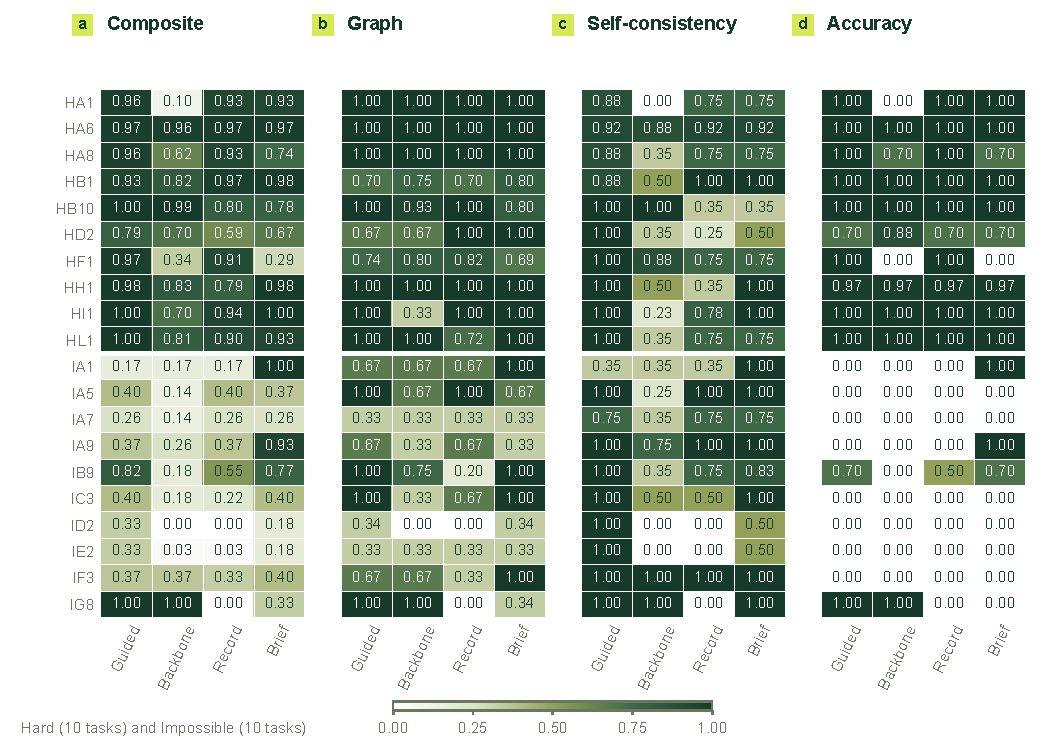
\includegraphics[width=\textwidth]{figures/bench_tasks_hi.pdf}
\caption{All Hard and Impossible task scores, with the same layer and configuration ordering as Figure~\ref{fig:si-task-matrix-en}. All 80 runs have complete composite and component values.}
\label{fig:si-task-matrix-hi}
\end{figure}
